\section{Galutinis rezultatas}

Čia bus pateikiamas gautas grafikas (žr.~\ref{fig:galutinis rezultatas} pav.).

\begin{figure}[H]
    \centering
    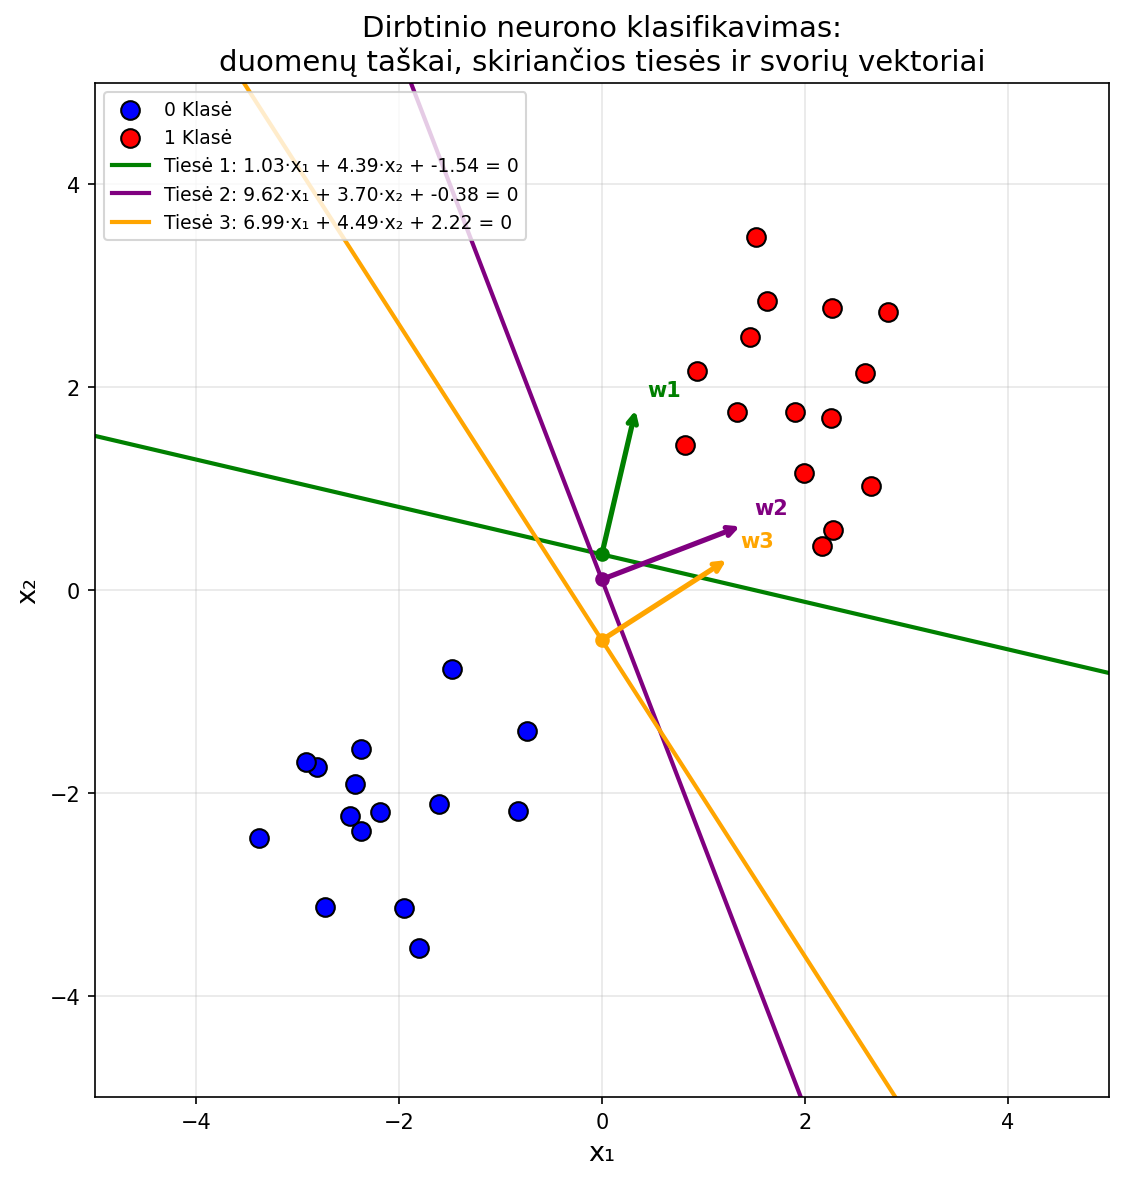
\includegraphics[scale=0.8]{../grafikai/neuronas.png}
    \caption{Duomenų taškai, klases skiriančios tiesės ir svorių vektoriai}
    \label{fig:galutinis rezultatas}
\end{figure}